%%%%%%%%%%%%%%%%%%%%%%%%%%%%%%%%%%%%%%%%%%%%%%%%%%%%%%%%%%%%%%%%%%%%%%
%%%%%%%%%%%%%%%%%%%%%%%%%%%%%%%%%%%%%%%%%%%%%%%%%%%%%%%%%%%%%%%%%%%%%%
\documentclass[dvips,portrait]{seminar}             %%%%%%%%%%%%%%%%%%
                                                    %%%%%%%%%%%%%%%%%%
%%%%%%%%%%%%%%%%%%%%%%%%%%%%%%%%%%%%%%%%%%%%%%%%%%%%
% gmake Sli-IFImu-ps
% pstops '1:0@0.925(10mm,-1mm)'  Sli-IFImu.ps   Sli-IFImu-redu.ps
%======================

%%%%%%%%%%%%%%%%%%%%%%%%%%%%%%%%%%%%%%%%%%%%%%%%%%%%%%%
%%%%%%%%%%%%%%%%%%%%%%%%%%%%%%%%%%%%%%%%%%%%%%%%%%%%%%%
\begin{document}                     %%%%%%%%%%%%%%%%%%


\def\title{\Color{PineGreen} TEST B, IFI}
\def\author{By \KK MC and ZFITTER teams}

%%%%%%%%%%%%%%%%%%%%%%%%%%%%%%%%%%%%%%%%%%%%%%%%%%%%%%%%%%%%%%%%%%%%%%%%%%%%%
%%%%%%%%%%%%%%%%%%%%%%%%%%%%%%%%%%%%%%%%%%%%%%%%%%%%%%%%%%%%%%%%%%%%%%%%%%%%%
%%%%%%%%%%%%%%%%%%%%%%%%%%%%%%%%%%%%%%%%%%%%%%%%%%%%%%%%%%%%%%%%%%%%%%%%%%%%%
\begin{slide*}                                                %%%%%%%%%%%%%%%
\titbox{{\large\Color{Magenta} \KK MC versus \KK sem, Zfitter}}
{\bf\color{blue}
\noindent
Summary table of x-sections for $\mu$-pairs. \\
QED FSR is on while IFI is on/off.\\
Simple cut $v=1-M^2_{inv}/s<v_{\max}$. Workshop input.\\
}

\begin{center}
\setlength{\unitlength}{1mm}
\begin{picture}(70,50)
%#####\put(0,0){\framebox( 65,60){ }}
\put(0,0){\makebox(0,0)[lb]{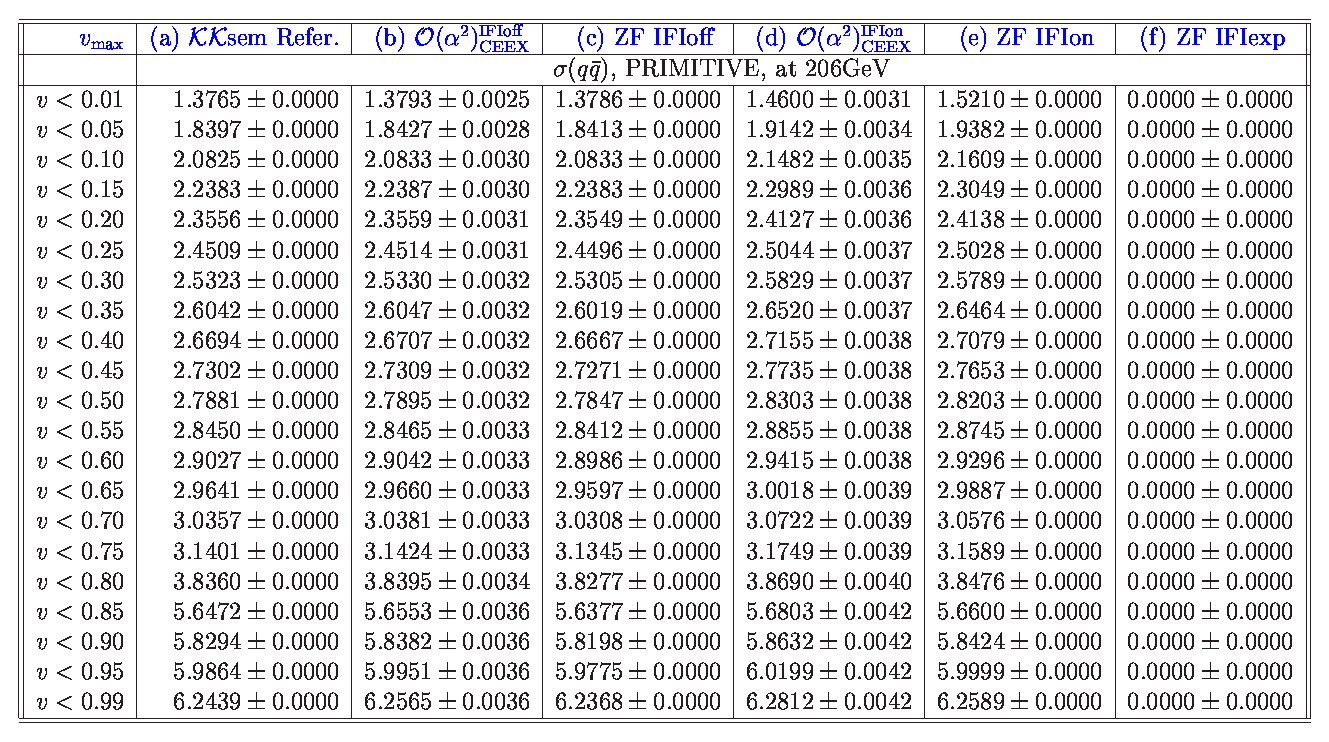
\epsfig{file=TabIFI-1.eps,width=70mm,height=50mm}}}
\end{picture}
\end{center}
\vspace{1mm}
\noindent
{\color{red} Remarks:
  see next slide.
}
\vfill
\end{slide*}   %%%
%%%%%%%%%%%%%%%%%%

%%%%%%%%%%%%%%%%%%%%%%%%%%%%%%%%%%%%%%%%%%%%%%%%%%%%%%%%%%%%%%%%%%%%%%%%%%%%%
%%%%%%%%%%%%%%%%%%%%%%%%%%%%%%%%%%%%%%%%%%%%%%%%%%%%%%%%%%%%%%%%%%%%%%%%%%%%%
%%%%%%%%%%%%%%%%%%%%%%%%%%%%%%%%%%%%%%%%%%%%%%%%%%%%%%%%%%%%%%%%%%%%%%%%%%%%%
\begin{slide*}                                                %%%%%%%%%%%%%%%
\titbox{{\large\Color{Magenta} \KK MC versus \KK sem, Zfitter}}
{\bf\color{blue}
\noindent
The same as in table in visual form. All for $\mu$-pairs. \\
Simple cut $v=1-M^2_{inv}/s<v_{\max}$. Workshop input.\\
Black dots are analytical result in soft limit, up to a constant.
}

\begin{center}
\setlength{\unitlength}{1mm}
\begin{picture}(80,40)
%%\put(0,0){\framebox( 80,80){ }}
\put(-2,0){\makebox(0,0)[lb]{\epsfig{file=FigFSR-Mu.eps,width=40mm,height=40mm}}}
\put(40,0){\makebox(0,0)[lb]{\epsfig{file=FigIFI-Mu.eps,width=40mm,height=40mm}}}
\end{picture}
\end{center}

{\Color{PineGreen}\small\bf Remarks:
  For IFI off we see now 0.2\% agreement \KK MC, KKsem and ZFITTER
  for typical Z-exclusive photon energy cut, 
  and 0.3\% for Z-inclusive!
  The same \KK-ZF agreement for IFI switched on.}

\vfill
\end{slide*}   %%%
%%%%%%%%%%%%%%%%%%



%%%%%%%%%%%%%%%%%%%%%%%%%%%%%%%%%%%%%%%%%%%%%%%%%%%%%%%%%%%%%%%%%%%%%%%%%%%%%
%%%%%%%%%%%%%%%%%%%%%%%%%%%%%%%%%%%%%%%%%%%%%%%%%%%%%%%%%%%%%%%%%%%%%%%%%%%%%
%%%%%%%%%%%%%%%%%%%%%%%%%%%%%%%%%%%%%%%%%%%%%%%%%%%%%%%%%%%%%%%%%%%%%%%%%%%%%
\begin{slide*}                                                %%%%%%%%%%%%%%%
\titbox{{\large\Color{Magenta} \KK MC versus \KK sem, Zfitter}}
{\bf\color{blue}
\noindent
Closer look at IFI itself in the cross section.
}

\begin{center}
\setlength{\unitlength}{1mm}
\begin{picture}(80,40)
%%\put(0,0){\framebox( 80,40){ }}
\put(-2, 0){\makebox(0,0)[lb]{\epsfig{file=FigIFI-Mu1.eps,width=40mm,height=40mm}}}
\put(40, 0){\makebox(0,0)[lb]{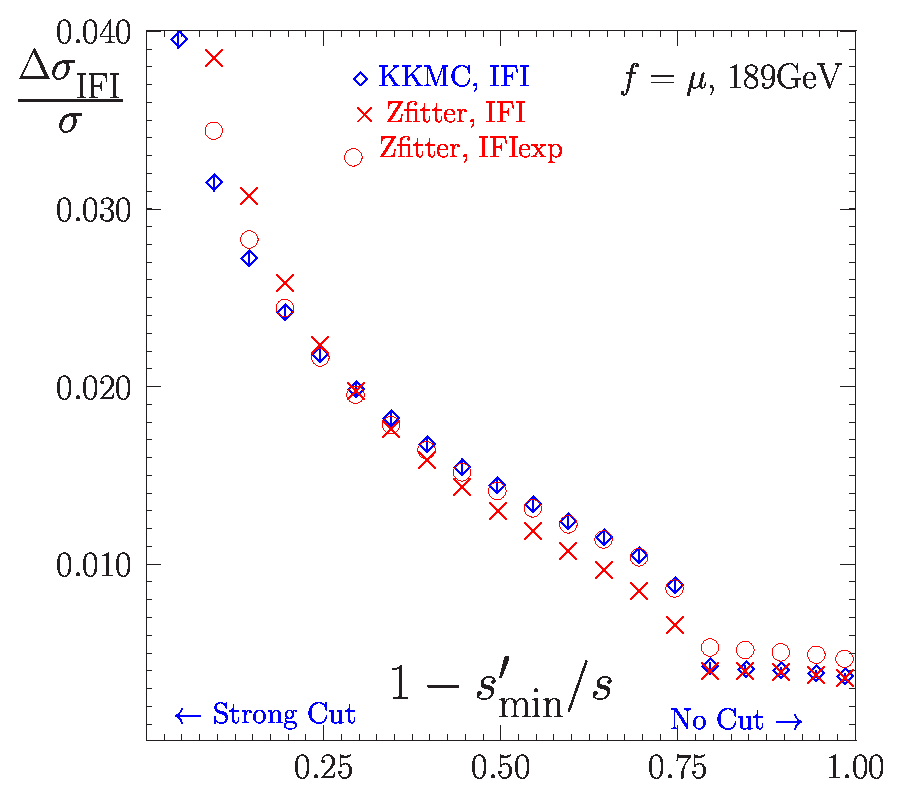
\epsfig{file=FigIFI-Mu2.eps,width=40mm,height=40mm}}}
\end{picture}
\end{center}

{\Color{PineGreen}\small\bf Remarks:
  For IFI itself the agreement \KK-ZF is up to 0.4\%
  for typical Z-exclusive and Z-inclusive photon energy cuts.
  The difference \KK-ZFexp is twice smaller, up to 0.2\%
}

\vfill
\end{slide*}   %%%
%%%%%%%%%%%%%%%%%%


%%%%%%%%%%%%%%%%%%%%%%%%%%%%%%%%%%%%%%%%%%%%%%%%%%%%%%%%%%%%%%%%%%%%%%%%%%%%%
%%%%%%%%%%%%%%%%%%%%%%%%%%%%%%%%%%%%%%%%%%%%%%%%%%%%%%%%%%%%%%%%%%%%%%%%%%%%%
%%%%%%%%%%%%%%%%%%%%%%%%%%%%%%%%%%%%%%%%%%%%%%%%%%%%%%%%%%%%%%%%%%%%%%%%%%%%%
\begin{slide*}                                                %%%%%%%%%%%%%%%
\titbox{{\large\Color{Magenta} \KK MC versus \KK sem, Zfitter}}
{\bf\color{blue}
\noindent
Asymmetry $A_{FB}$ without IFI.
}

\begin{center}
\setlength{\unitlength}{1mm}
\begin{picture}(80,40)
%%\put(0,0){\framebox( 80,40){ }}
\put(-2, 0){\makebox(0,0)[lb]{\epsfig{file=FigFSR-MuAfb.eps,width=40mm,height=40mm}}}
\put(40, 0){\makebox(0,0)[lb]{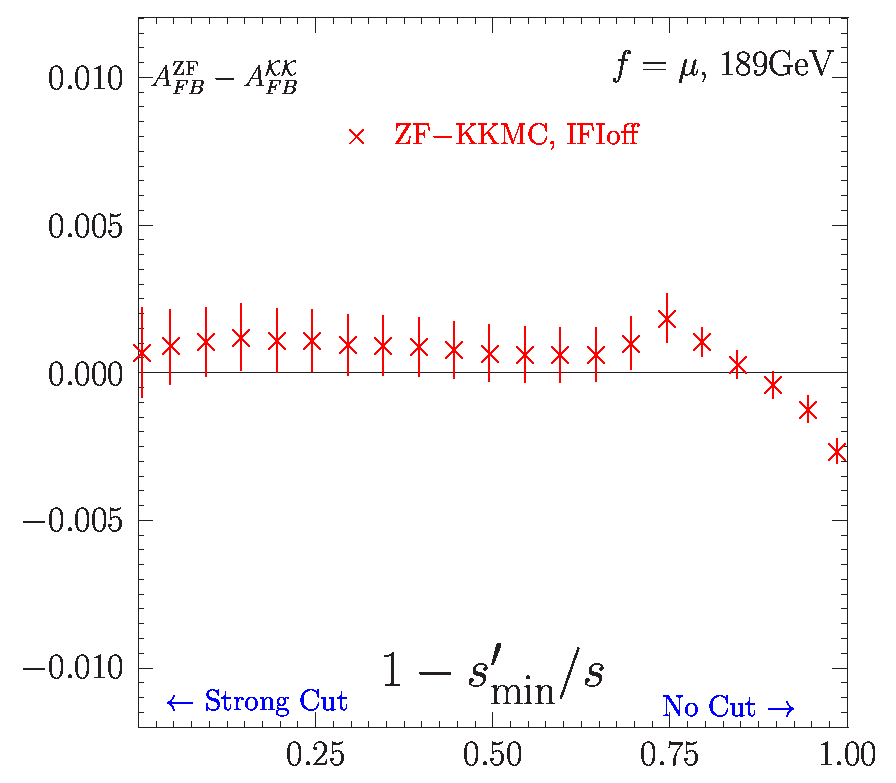
\epsfig{file=FigFSR-MuAfb1.eps,width=40mm,height=40mm}}}
\end{picture}
\end{center}

{\Color{PineGreen}\small\bf Remarks:
  Without IFI the difference \KK-ZF In $A_{FB}$ is up to a satisafctory 0.25\% everywhere.
  Both for typical Z-exclusive and Z-inclusive photon energy cuts.
}

\vfill
\end{slide*}   %%%
%%%%%%%%%%%%%%%%%%


%%%%%%%%%%%%%%%%%%%%%%%%%%%%%%%%%%%%%%%%%%%%%%%%%%%%%%%%%%%%%%%%%%%%%%%%%%%%%
%%%%%%%%%%%%%%%%%%%%%%%%%%%%%%%%%%%%%%%%%%%%%%%%%%%%%%%%%%%%%%%%%%%%%%%%%%%%%
%%%%%%%%%%%%%%%%%%%%%%%%%%%%%%%%%%%%%%%%%%%%%%%%%%%%%%%%%%%%%%%%%%%%%%%%%%%%%
\begin{slide*}                                                %%%%%%%%%%%%%%%
\titbox{{\large\Color{Magenta} \KK MC versus \KK sem, Zfitter}}
{\bf\color{blue}
\noindent
Asymmetry  $A_{FB}$ with IFI contribution,\\
 and the difference \KK-ZF.
}

\begin{center}
\setlength{\unitlength}{1mm}
\begin{picture}(80,40)
%%\put(0,0){\framebox( 80,40){ }}
\put(-2, 0){\makebox(0,0)[lb]{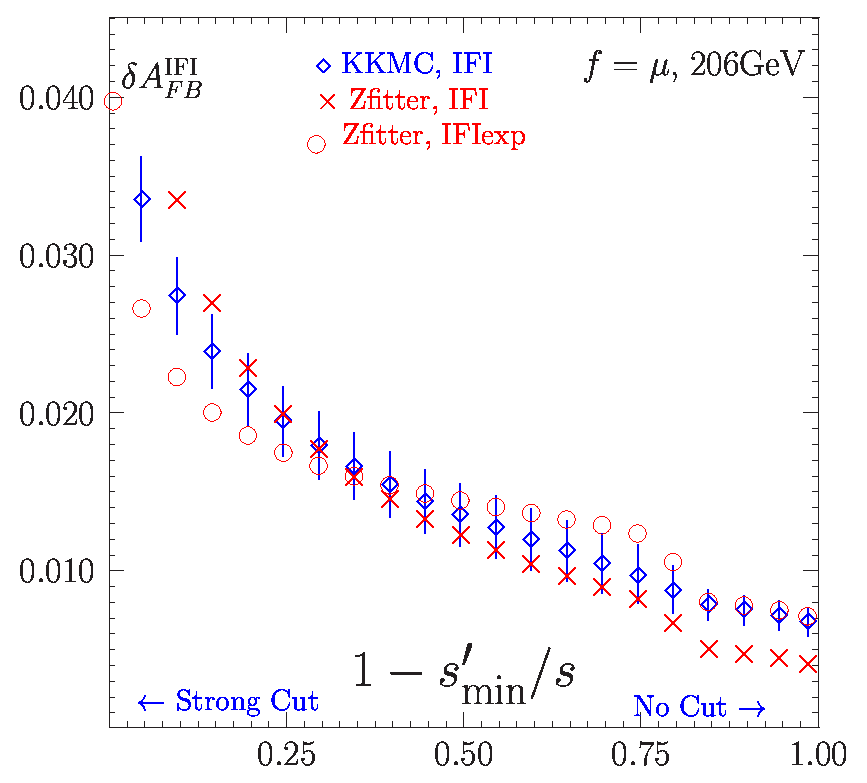
\epsfig{file=FigIFI-MuAfb2.eps,width=40mm,height=40mm}}}
\put(40, 0){\makebox(0,0)[lb]{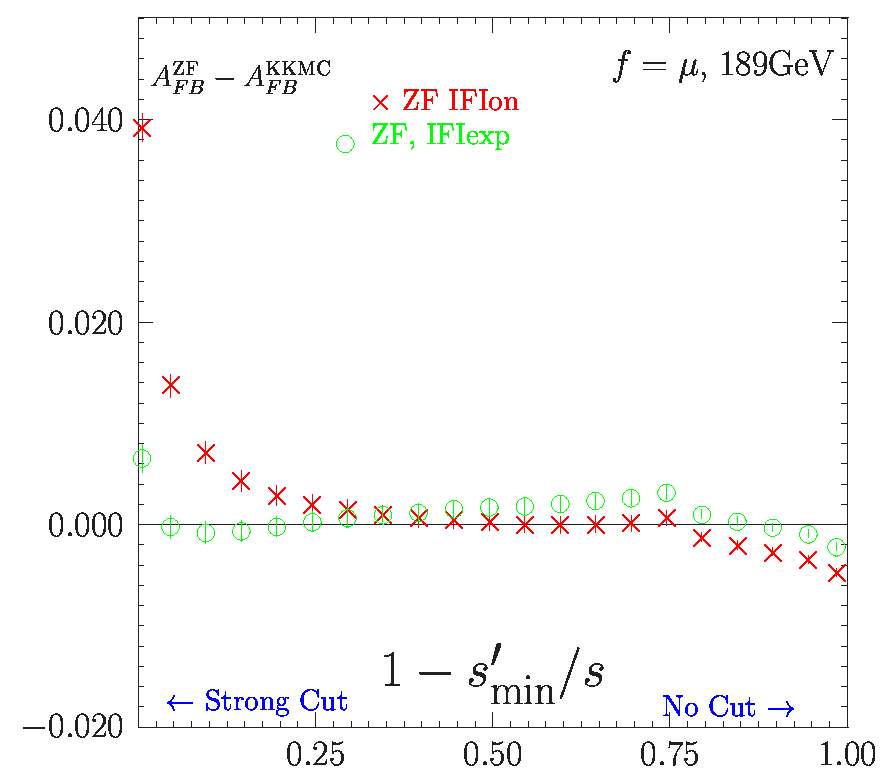
\epsfig{file=FigIFI-MuAfb1.eps,width=40mm,height=40mm}}}
\end{picture}
\end{center}

{\Color{PineGreen}\small\bf Remarks:
  For IFI corr. to $A_{FB}$ the difference \KK-ZF is up to 0.25\%
  for typical Z-exclusive and Z-inclusive photon energy cuts.
  The difference \KK-ZFexp is smaller, especially in soft limit.
}

\vfill
\end{slide*}   %%%
%%%%%%%%%%%%%%%%%%

\end{document}

